\documentclass[
    english, % Klasei padavus parametrą 'english', darbas bus anglų kalba.
    % signatureplaces % prideda parašų vietas tituliniame puslapyje
]{VUMIFPSkursinis}
\usepackage{float}
\usepackage{wrapfig2}
\usepackage{hyperref}
\usepackage{algorithmicx}
\usepackage{algorithm}
\usepackage{algpseudocode}
\usepackage{amsfonts}
\usepackage{amsmath}
\usepackage{bm}
\usepackage{caption}
\usepackage{color}
\usepackage{graphicx}
\usepackage{listings}
\usepackage{subcaption}
\usepackage{biblatex}
\usepackage[inkscapelatex=false]{svg}


% Titulinio aprašas
\university{Vilnius university}
\faculty{Faculty of mathematics and informatics}
\department{Software engineering study program}
\papertype{Software Engineering II laboratory work 2}
\title{EduPal system architecture}
\status{2 course 5 group students}
\author{Motiejus Šveikauskas}
\secondauthor{Kanstantinas Piatrashka}
\thirdauthor{Aldas Vertelis}
\fourthauthor{Danielius Podbielski}
\reviewer{doc. dr. Vardauskas Pavardauskas}
\date{Vilnius – \the\year}

\bibliography{bibliografija}

\begin{document}
\maketitle

\tableofcontents

\sectionnonum{Įvadas}
Įvade apibūdinamas darbo tikslas ir t.t., temos aktualumas ir siekiami rezultatai.
Darbo įvadas neturi būti dėstymo santrauka. Įvado apimtis 1–-2 puslapiai.
\includesvg[width=\textwidth]{../lab2diags/LogicalView/Logical_viewsvg.drawio}

\section{Medžiagos darbo tema dėstymo skyriai}
Medžiagos darbo tema dėstymo skyriuose pateikiamos nagrinėjamos temos detalės:
pradinė medžiaga, jos analizės ir apdorojimo metodai, sprendimų įgyvendinimas,
gautų rezultatų apibendrinimas. Šios dalies turinys labai priklauso nuo darbo
temos. Skyriai gali turėti poskyrius ir smulkesnes sudėtines dalis, kaip
punktus ir papunkčius.

Medžiaga turi būti dėstoma aiškiai, pateikiant argumentus. Tekste dėstomas
trečiuoju asmeniu, t.y. rašoma ne \enquote{aš manau}, bet „autorius mano“, „autoriaus
nuomone“. Reikėtų vengti informacijos nesuteikiančių frazių, pvz., „...kaip jau
buvo minėta...“, \enquote{...kaip visiems žinoma...} ir pan., vengti grožinės
literatūros ar publicistinio stiliaus, gausių metaforų ar panašių meninės
išraiškos priemonių.

Skyriai gali turėti poskyrius ir smulkesnes sudėtines dalis, kaip punktus ir
papunkčius.

\subsection{Poskyris}
Citavimo pavyzdžiai: cituojamas vienas šaltinis \cite{PvzStraipsnLt}; cituojami
keli šaltiniai \cite{PvzStraipsnEn, PvzStraipsnLta, PvzKonfLt, PvzKonfEn, PvzKnygLt, PvzKnygEn,
    PvzElPubLt, PvzElPubEn, PvzBakLt, PvzMagistrLt, PvzPhdEn}.

Anglų kalbos terminų pateikimo pavyzdžiai: priklausomybių injekcija (\anglnb{dependency injection},
dažnai trumpinama kaip \textit{DI}), saitų redaktorius \angl{linker}.

Išnašų\footnote{Pirma išnaša.} pavyzdžiai\footnote{Antra išnaša.}.

\subsection{Faktorialo algoritmas}

\ref{alg:factorial} algoritmas parodo, kaip suskaičiuoti skaičiaus faktorialą.

\begin{algorithm}
    \caption{Skaičiaus faktorialas}
    \begin{algorithmic}[1] % [1] padaro, kad eilutės būtų sunumeruotos
        \State $N\gets$ skaičius, kurio faktorialą skaičiuojame
        \State $F\gets 1$
        \For{$i := 2$ to $N$}
        \State $F\gets F \cdot i$
        \EndFor
    \end{algorithmic}
    \label{alg:factorial}
\end{algorithm}

\subsubsection{Punktas}
\subsubsubsection{Papunktis}
\subsubsection{Punktas}
\section{Skyrius}
\subsection{Poskyris}
\subsection{Poskyris}

\sectionnonum{Rezultatai ir išvados}
Rezultaas ir išvadų dalyje turi būti aiškiai išdėstomi pagrindiniai darbo
rezultatai (kažkas išanalizuota, kažkas sukurta, kažkas įdiegta) ir pateikiamos
išvados (daromi nagrinėtų problemų sprendimo metodų palyginimai, teikiamos
rekomendacijos, akcentuojamos naujovės).

\sectionnonum{Išvados}
\begin{enumerate}[labelindent=0pt]
    \item Išvadų skyriuje daromi nagrinėtų problemų sprendimo metodų palyginimai, siūlomos
          rekomendacijos, akcentuojamos naujovės.
    \item Išvados pateikiamos sunumeruoto (gali būti hierarchinis) sąrašo pavidalu.
    \item Darbo išvados turi atitikti darbo tikslą.
\end{enumerate}

\printbibliography[heading=bibintoc]  % Šaltinių sąraše nurodoma panaudota
% literatūra, kitokie šaltiniai. Abėcėlės tvarka išdėstomi darbe panaudotų
% (cituotų, perfrazuotų ar bent paminėtų) mokslo leidinių, kitokių publikacijų
% bibliografiniai aprašai. Šaltinių sąrašas spausdinamas iš naujo puslapio.
% Aprašai pateikiami netransliteruoti. Šaltinių sąraše negali būti tokių
% šaltinių, kurie nebuvo paminėti tekste (LaTeX tai sutvarko automatiškai).

% \sectionnonum{Sąvokų apibrėžimai}
\sectionnonum{Santrumpos}
Sąvokų apibrėžimai ir santrumpų sąrašas sudaromas tada, kai darbo tekste
vartojami specialūs paaiškinimo reikalaujantys terminai ir rečiau sutinkamos
santrumpos.

% Priedai
% Prieduose gali būti pateikiama pagalbinė, ypač darbo autoriaus savarankiškai
% parengta, medžiaga. Savarankiški priedai gali būti pateikiami ir
% kompaktiniame diske. Priedai taip pat numeruojami ir vadinami. Darbo tekstas
% su priedais susiejamas nuorodomis.
\appendix{Neuroninio tinklo struktūra}

\begin{figure}[H]
    \centering
    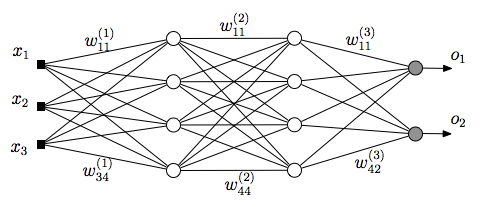
\includegraphics[scale=0.5]{img/MLP}
    \caption{Paveikslėlio pavyzdys}
    \label{img:mlp}
\end{figure}


\appendix{Eksperimentinio palyginimo rezultatai}

% tablesgenerator.com - converts calculators (e.g. excel) tables to LaTeX
\begin{table}[H]\footnotesize
    \centering
    \caption{Lentelės pavyzdys}
    {\begin{tabular}{|l|c|c|} \hline
            Algoritmas   & $\bar{x}$ & $\sigma^{2}$ \\
            \hline
            Algoritmas A & 1.6335    & 0.5584       \\
            Algoritmas B & 1.7395    & 0.5647       \\
            \hline
        \end{tabular}}
    \label{tab:table example}
\end{table}

\end{document}
